%%
% ----------------------------------------------------------------------------
% "THE BEER-WARE LICENSE" (Revision 42):
% <sebastian.rauh@hs-heilbronn.de/michael.bauer@hs-heilbronn.de> wrote this 
% file. As long as you retain this notice you can do whatever you want with 
% this stuff. If we meet some day, and you think this stuff is worth it, you 
% can buy us a beer in return. 
% Michael Lukas Bauer, Sebastian Felix Rauh
% ----------------------------------------------------------------------------
%%

Die in Kapitel 3 aufgeführten Analyse Ergebnisse wurden für die erste Interation des Prototyps umgesetzt. Es handelt sich hierbei um ein funktionsfähigen Prototypen, der nativ auf der Apple Watch ausführbar ist. Im folgenden werden Schritte der Umsetzung genauer beschrieben. Hierbei wird genauer auf die Benutzeroberflächenerstellung, sowie auch die Verbindung zischen Uhr und iPhone eingegangen.

\section{Benutzeroberfläche}
Xcode bietet für visuelle Erstellung von Benutzeroberflächen ein eigenen integrierten Editor namens InterfaceBuilder bereit. Hiermit können graphische Elemente per DragAndDrop zu einer Benutzeroberfläche zusammengestellt werden \ref{fig:xcode-interface-elements}. Ebenfalls per DragAndDrop werden diese Inerface-Elemete mit dem Quellcode verbunden\ref{fig:xcode-interface-code-connect}.
\begin{figure}
	\caption{Interface Elemente zu Erstellen von Benutzeroberflächen}
	\label{fig:xcode-interface-elements}
	\centering
		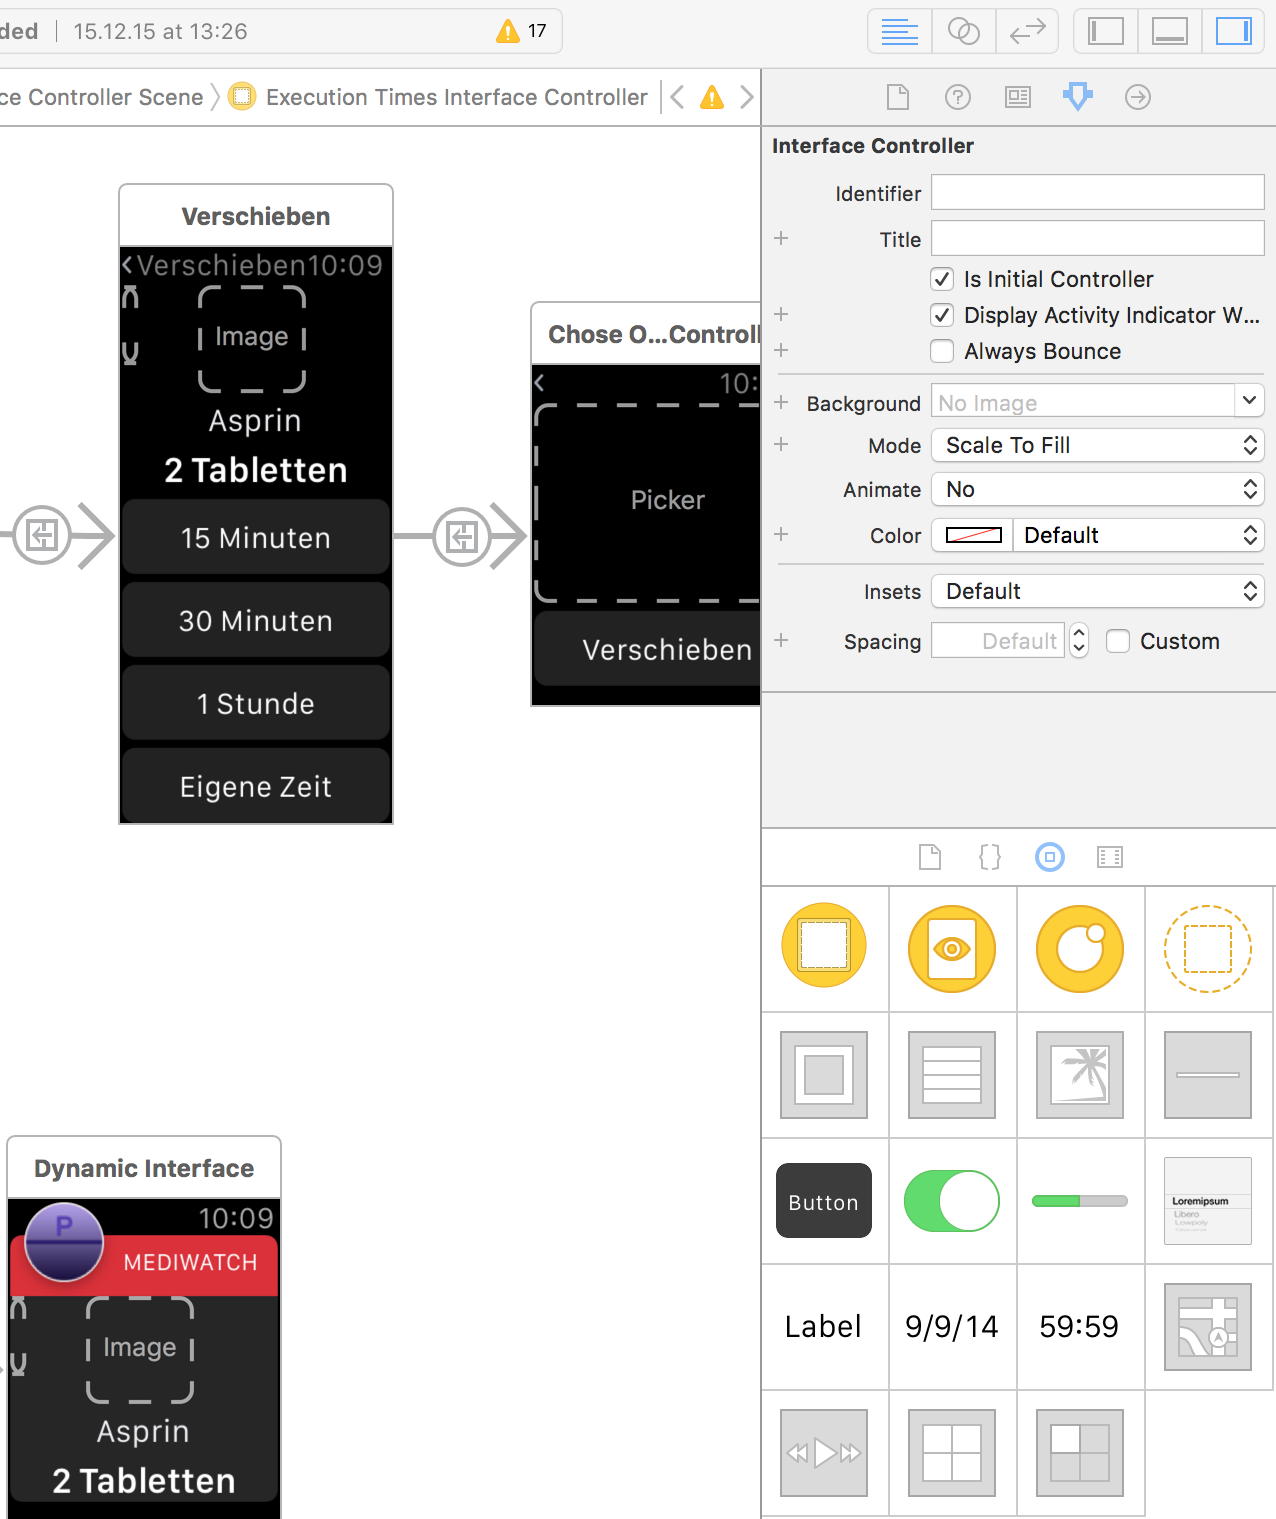
\includegraphics[width=0.9\textwidth]{04_realisation/screenshots/xcode-interface-elements}
\end{figure}

\begin{figure}
	\caption{Interface Elemente mit Quellcode verknüfen}
	\label{fig:xcode-interface-code-connect}
	\centering
	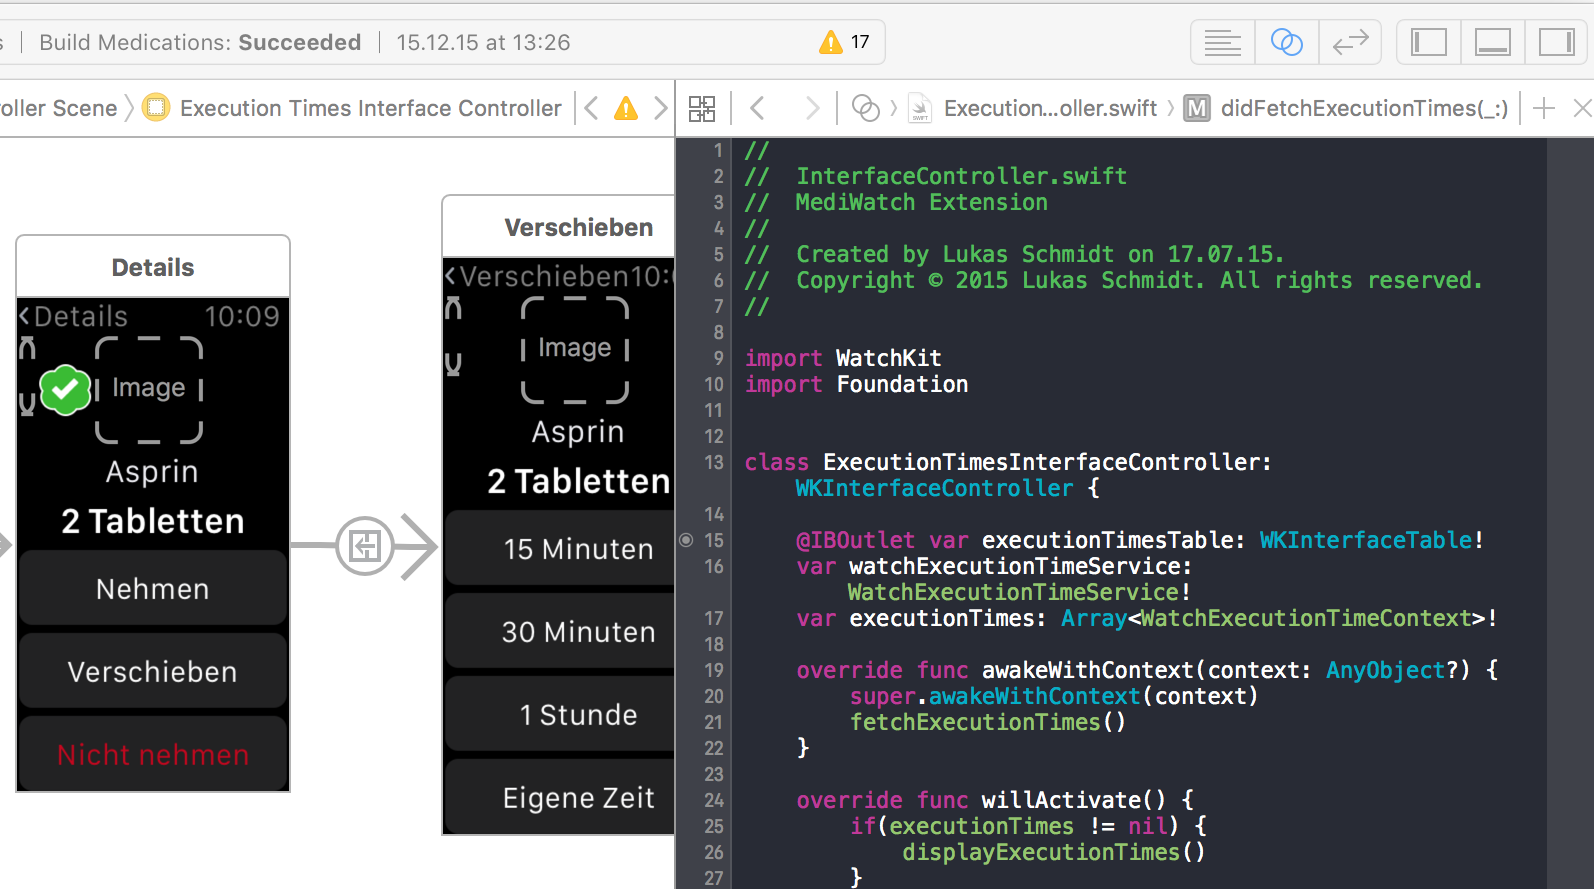
\includegraphics[width=0.9\textwidth]{04_realisation/screenshots/xcode-interface-code-connect}
\end{figure}

\section{WatchConnectivity}
Wichtig für die Kommunikation zwischen Uhr und iPhone ist das WatchConnectivity Framework. Hierbei ist ist im Listing xx zu sehen, wie genau eine Verbindung aufgebaut werden kann. Wichtig ist, das diese Verbindung zum richtigen Zeitpunkt im Application-Lifecycle aufgebaut wird, da es sonst zu Datenverlusten kommen kann.
\lstinputlisting[caption=Beispiel zu Type Inference in Swift label=lst:watchConnectifity]{04_realisation/code/WatchExecutionTimeService.swift}


\section{Anwendung}
